\newpage
\section{RPL}\label{sec:state-rpl}
\renewcommand{\rightmark}{RPL}
%TODO tour des protocoles de routages ??

Routing Protocol for Low-Power and Lossy Networks~\cite{rfc:rpl} est un protocole de routage IPv6 destiné aux réseaux dont les noeuds sont contraints en énergie et dont les liens sont soumis à des pertes importantes de paquets (Low-power and Lossy Networks, LLNs).

D'après l'article de Tripathi, Oliveira et Vasseur~\cite{paper:rpl-study}, après avoir été étudiés par le groupe de travail IETF roll (Routing Over Low power and Lossy networks), il s'est avéré que les protocoles tel que OSPF, AODV ou OLSR ne satisfont pas toutes les exigences des LLNs. C'est pour cette raison que ce groupe de travail a introduit RPL.
Ce protocole à vecteur de distance est un protocole proactif, c'est à dire que les routes sont établies avant qu'elles ne soient nécessaires.

RPL sépare le traitement et la transmission des paquets de contrôle de l'optimisation de l'objectif de routage. Cela permet de l'adapter à un large éventail d'applications des LLNs comme la domotique, l'automatisation industriel ou encore la récolte de données dans divers environnements.

%De plus, de part sa topologie et son fonctionnement, RPL est optimisé pour la collecte de données %ce qui est l'utilisation principale pour ce mémoire.

Cette section décrit le fonctionnement de RPL. Cette description est basée sur le RFC 6550~\cite{rfc:rpl}.


\subsection*{Topologie}
    RPL construit un DODAG (Destination Oriented Directed Acyclic Graph) qui est un graphe dirigé 
    acyclique (DAG) ayant une seule racine (Fig.~\ref{fig:state-dodag}). De par cette architecture 
    RPL est adapté aux applications de collecte de données ce qui est le principale objectif de ce 
    projet. En effet, la route d'un noeud à la racine est facilement établie car tous les noeuds du 
    chemins envoient les données à leur parent.

    \begin{figure}[H]
        \centering
        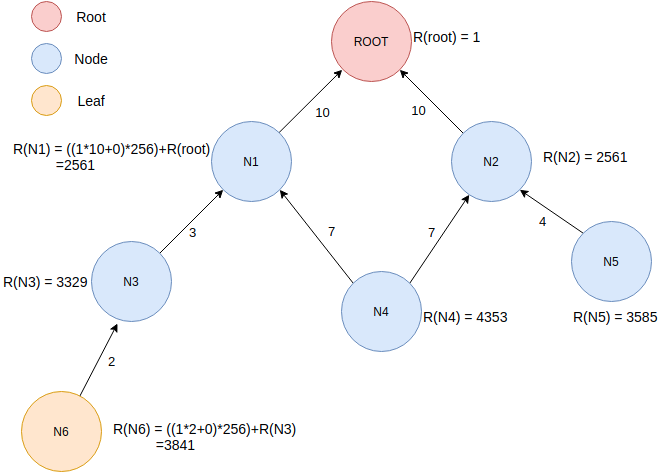
\includegraphics[scale=0.45]{res/pictures/dodag.drawio.png}
        \caption{DODAG.}
        \label{fig:state-dodag}
    \end{figure}


\subsection*{Fonctions objectif}
Une fonction objectif (OF) définit comment plusieurs métriques sont utilisées pour calculer le rang d'un noeud. Celui-ci détermine la position du noeud dans le DODAG par rapport aux autres noeuds.
Le rang augmente strictement dans le sens descendant et diminue strictement dans le sens montant. Ainsi, pour un noeud $n$, la propriété $rang(n)>rang(parent(n))$ est toujours vérifiée. La figure~\ref{fig:state-dodag} illustre un DODAG avec des valeurs de rang calculées avec la fonction objectif OF0, ses paramètres par défaut et des coûts de liens attribués administrativement. Sur cet exemple, la racine du DODAG a comme rang, la valeur par défaut $\textsc{root\_rank}=1$ définie dans le RFC 6550.

Les fonctions objectif OF0 et MRHOF, implémentées dans Contiki, sont décrites sur base du RFC 6552~\cite{rfc:of0} et du RFC 6719 ~\cite{rfc:mrhof}.

    \subsubsection*{OF0}
        \textit{Objective Function Zero} est une fonction dont l'objectif est de choisir un parent qui permettra à un noeud d'être le plus proche possible la racine du DODAG.
        Le calcul du rang d'un noeud $N$, $R(N)$, est décrit par l'équation~\ref{eq:state-rankOF0}. Il est calculé pour chaque parent potentiel. Le parent préféré choisi sera alors le parent potentiel qui implique le plus petit $R(N)$.\par


        Le calcul du rang commence par le calcul de la variable \textit{step\_of\_rank} ($Sp$) qui est 
        basée sur  les propriétés et métriques du lien avec le parent potentiel. Le RFC 
        recommande de baser ce calcul sur des propriétés dynamiques comme la métrique \textit{expected transmission count (ETX)} décrit dans l'article de Couto, Aguayo, Bicket et Morris
        ~\cite{paper:etx}, qui est une métrique qui permet de minimiser le nombre de transmissions requises pour transmettre un paquet.
        L'utilisation de propriétés dynamiques est recommandée car utiliser des propriétés statiques, comme un coût administratif, revient à avoir un
        rang analogue au nombre de sauts. 
        
        $Sp$ est ensuite mutlipliée par la variable \textit{rank\_factor} ($Rf$) qui est utilisée pour multiplier son effet dans le calcul de
        \textit{rank\_increase}. $Rf$ doit être un entier strictement positif et sa valeur par défaut est 1.

        $Sr$ est un terme plus petit ou égal à la variable \textit{stretch\_of\_rank} qui est l'augmentation maximum de \textit{step\_of\_rank} avec le parent.


        La variable \textit{rank\_increase} est finalement multipliée par le facteur \textit{MinHopRankIncrease} qui est défini par le RFC 6550~\cite{rfc:rpl} comme l'augmentation minimum du rang entre un noeud et n'importe lequel de ses parents. Sa valeur par défaut est \textsl{\textsc{default\_min\_hop\_rank\_increase}} qui a une valeur de 256.
        
        Le calcul du rang est la somme du rang du parent potentiel $P$, $R(P)$, et de \textit{rank\_increase}.

        \begin{equation}\label{eq:state-rankOF0}
            \begin{aligned}
                rank\_increase &= (Rf * Sp + Sr) * MinHopRankIncrease\\
                R(N) &= R(P) + rank\_increase    
            \end{aligned}
        \end{equation} 
        %Le rang d'un noeud $R(N)$ est calculé comme suit:
        %    \[rank\_increase = (Rf * Sp + Sr) * MinHopRankIncrease\]
        %    \[R(N) = R(P) + rank\_increase\]
        %    où
        %    \begin{itemize}
        %        \item $Rf$ est le $rank\_factor$ et $Sr \leq stretch\_of\_rank$ avec %$rank\_factor$ et $stretch\_of\_rank$ deux paramètres de la fonction
        %        
        %        \item $Sp$ est le $step\_of\_rank$ qui est une valeur basée sur les propriétés %du lien. 
        %        
        %        \item $MinHopRankIncrease$ est une constante
        %        
        %        \item $R(P)$ est le rang d'un parent $p$
        %    \end{itemize}
        %    $R(N)$ est calculé pour chaque parent potentiel. Le parent préféré choisi sera %alors le parent potentiel qui implique le plus petit $R(N)$.
                
    \subsubsection*{MRHOF}%rfc6719
            \textit{Minimum Rank with Hysteresis Objective Function} est une fonction dont l'objectif est de sélectionner les routes qui minimisent une métrique additive en utilisant l'hystérésis
            pour réduire les changements de parents en réponse a de petites variations de la métrique.
            
            Pour cela, un noeud va calculer le coût des chemins avec chaque candidat parent. Ce coût sera la somme de deux éléments:
            \begin{itemize}
                \item La valeur de la métrique utilisée contenue dans les DIOs d'un candidat parent
                \item La valeur de la métrique pour le lien entre ce noeud et le candidat parent
            \end{itemize}
            Si le coût d'un chemin est plus grand qu'une constante \textsl{\textsc{max\_link\_metric}} dont la valeur recommandée par le RFC 6719~\cite{rfc:mrhof} est 512,
            le noeud va exclure le candidat parent utilisant ce lien.
            Un noeud va choisir comme parent le candidat parent pour lequel le coût du chemin est le plus petit. Le changement de parent ne s'effectue que si la condition suivante est satisfaite:
            \[ |cost-old\_cost| > \textsc{parent\_switch\_treshold} \]
            Le RFC 6719 recommande 192 comme valeur pour \textsl{\textsc{parent\_switch\_treshold}} si la métrique utilisée est ETX.

\subsection*{Messages RPL}
    RPL défini quatre types de mesages de contrôles: DIO, DIS, DAO et DAO-ACK. Ces messages de contôles sont des messages ICMPv6. Le RFC 6550~\cite{rfc:rpl} indique que ces messages ont la portée d'un lien, à l'exception des DAO/DAO-ACK qui dans le mode de fonctionnement \textit{non-storing} sont envoyés en unicast et donc utilisent des adresse unique-local ou global. Pour tous les autres messages, les adresses sources sont des adresses link-local et les adresses de destination sont soit link-local, soit l'adresse multicast pour tous les noeuds RPL qui est \texttt{ff02::1a}.

\subsubsection*{DIO}
    Les DIOs (DODAG Information Object) annoncent des informations sur le DODAG qui permettent aux noeuds de découvrir une instance RPL, de sélectionner un parent ou encore de maintenir le DODAG.
    Un DIO, illustré à la figure~\ref{fig:state-dio}, inclu notamment les champs suivants:
    \begin{itemize}
        \item InstanceID: Identifie l'instance RPL du DODAG
        \item Rank: Le rang du noeud qui émet le DIO
        \item MOP (Mode of Operation): Le mode d'opération de l'instance RPL (c.f. \fullref{subsec:state-mop}).
        \begin{enumerate}
            \setcounter{enumi}{-1}
            \item Pas de routes descendantes
            \item Non-storing mode
            \item Storing mode sans multicast
            \item Storing mode avec multicast
        \end{enumerate}
        \item DODAGID: Adresse IPv6 définie par la racine qui identifie le DODAG
    \end{itemize}
    \begin{figure}[H]
        \centering
        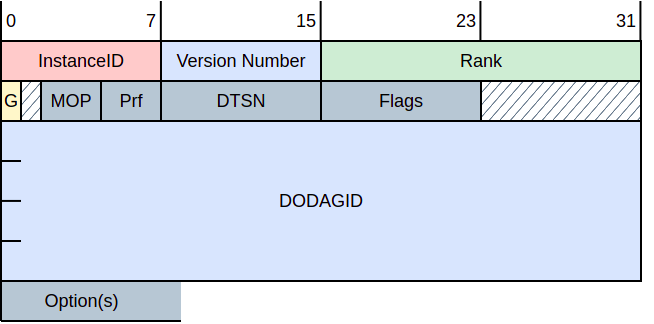
\includegraphics[scale=0.5]{res/pictures/dio.drawio.png}
        \caption{DODAG Information Object.}
        \label{fig:state-dio}
    \end{figure}

    Les DIOs sont transmis en utilisant l'algorithme Trickle~\cite{rfc:trickle}. Cet algorithme permet de réduire la quantité de messages envoyés en réduisant les transmissions quand les conditions sont stables et en les augmentant lorsque qu'un changement est observé dans le réseau.

\subsubsection*{DIS}
    Les DODAG Information Solicitation (DIS) sont utilisés pour soliciter un DIO d'un noeud RPL.

\subsubsection*{DAO}%p42
    Les DAOs (Destination Advertisement Object) sont utilisés pour établir les routes descendantes.
    Ils sont donc envoyés vers le haut du DODAG. Le format du DAO est illustré à la figure~\ref{fig:state-dao}. Un DAO est composé des champs suivants:
    \begin{itemize}
        \item InstanceID: identifie l'instance du DODAG
        \item K: indique que le destinataire doit répondre avec un DAO-ACK
        \item D: indique que le DODAGID est présent
        \item DAOSequence: Incrémenté à chaque DAO d'un noeud et répété dans le DAO-ACK
        \item DODAGID (optionnel)
    \end{itemize}
    \begin{figure}[H]
        \centering
        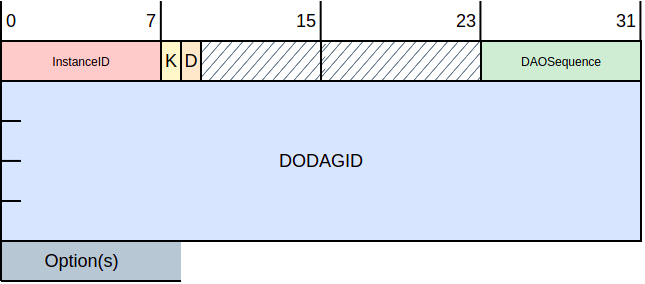
\includegraphics[scale=0.5]{res/pictures/dao.drawio.png}
        \caption{DODAG Information Object.}
        \label{fig:state-dao}
    \end{figure}

\subsubsection*{DAO-ACK}
    Le format d'un DAO-ACK est similaire à celui d'un DAO. Il n'est donc pas utile de le décrire.

\subsection*{Construction du réseau}
    La construction d'un DODAG est réalisée via l'échange de messages DIOs pour les routes montantes et de DAOs pour les routes descendantes. La figure~\ref{fig:state-dio-dao} illustre l'échange de ces messages.

\subsubsection*{Routes Montantes}
    %rfc: p 16, 19, 66
    Les routes montantes sont construites et maintenues avec les DIOs.
    L'algorithme de construction du DODAG est le suivant:
    \begin{enumerate}
        \item Les noeuds étant configurés comme racine d'un DODAG diffusent des DIOs en multicast à tous les noeuds RPL
        \item Les noeuds voulant rejoindre un DODAG écoutent ces DIOs et utilisent leurs informations pour rejoindre le DODAG (i.e. sélectionner un parent) ou maintenir le DODAG existant en accord avec la fonction objectif
        \item Les noeuds rajoutent des entrées dans leur table de routage pour les destinations spécifiées dans le DIO via leurs parents
        \item Une fois qu'un noeud a rejoint le DODAG, il diffuse à son tour des DIOs pour que d'autres noeuds puissent rejoindre le DODAG.
    \end{enumerate}

    Les noeuds qui opèrent comme feuille peuvent émettre des DIOs mais le rang contenu dans le DIO doit être l'infini. De cette manière une feuille ne sera pas choisie comme parent.

    Si une adresse de destination n'appartient pas au DODAG, la racine du DODAG peut transférer les paquets à l'exterieur de ce réseau, ou, si elle n'en est pas capable, les ignorer.     

\subsubsection*{Routes Descendantes}
    %rfc: p 19
    Les routes descendantes sont construites et maintenues avec les DAOS.
    L'échange des DAOs différe selon le mode de fonctionnement (MOP) du réseau. Ces différences sont détaillées en \fullref{subsec:state-mop}.

\begin{figure}[H]
    \centering
    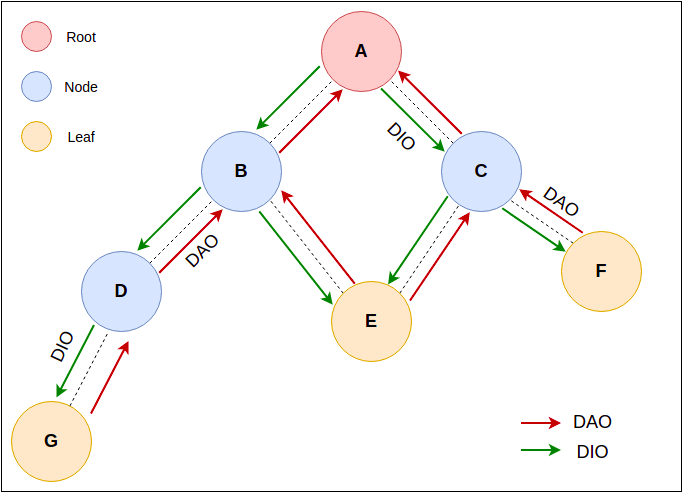
\includegraphics[scale=0.5]{res/pictures/dao-dio.drawio.png}
    \caption{Propagation des DIOs et DAOs.}
    \label{fig:state-dio-dao}
\end{figure}

%\subsection{Maintenance du réseau}


\subsection*{Modes de fonctionnements}\label{subsec:state-mop}
    %RFC p 19,20,41,77,78
    Le mode de fonctionnement d'une instance RPL, est défini administrativement et est annoncé par la racine. Les modes suivants sont disponibles:
    \begin{itemize}
        \item \textbf{Pas de routes descendantes}\\
            RPL ne maintient pas de routes descendantes. Dans ce MOP, les DAOs ne sont pas émis par les noeuds d'un DODAG, et les noeuds ignorent les DAOs.
        \item \textbf{Non-storing mode}\\
            Dans ce mode, les DAOs sont envoyés en unicast à la racine du DODAG.
            Les noeuds ne stockent pas de routes descendantes.
            
            %--new
            L'envoi des paquets le long de ces routes se fait donc par source-routing. Cela signifie qu'une en-tête de routage est ajoutée aux datagrammes par la racine. Le RFC 6554~\cite{rfc:rpl-routing-header} défini les mécanismes liés à ce type d'en-tête ainsi que son format qui est similaire à celui de l'en-tête de routage IPv6~\cite{rfc:ipv6} (de Type 0). Toutefois, il introduit en plus un mécanisme qui permet de compresser les adresses quand elles ont toutes le même préfixe.

            Dans ce mode, les paquets remontent donc jusqu'à la racine, qui rajoute l'en-tête de routage pour ensuite redescendre jusqu'au noeud de destination (Fig.~\ref{fig:state-path-nonstoring}).
            %--old
            %Donc les routes sont établies par source routing. C'est à dire que les paquets %remontent jusqu'à la racine du DODAG qui place dans les paquets tous les sauts de la %route pour ensuite redescendre (Fig.~\ref{fig:state-path-nonstoring}).
            %source/dest DAO unique-local ou global
            %--
        \item \textbf{Storing mode}\\
            Le storing mode peut être utilisé avec ou sans multicast.
            Dans ce mode, les DAOs sont envoyées en unicast par les noeuds à leur parent.
            Les paquets remontent jusqu'à un ancêtre commun avec la destination avant de redescendre vers celle-ci (Fig.~\ref{fig:state-path-storing}).
            Les noeuds stockent les routes de leur sous DODAG. Ainsi, chaque saut dans un chemin examine sa table de routage pour choisir le saut suivant.
            %source et destination des DAO: link-local
    \end{itemize}
    
    \begin{figure}[H]
        \centering
        \begin{subfigure}[b]{0.45\textwidth}
            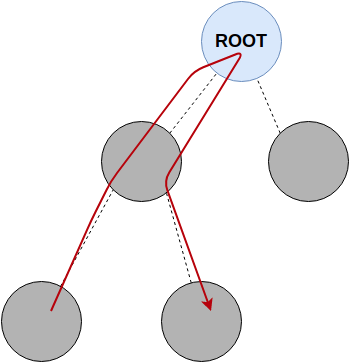
\includegraphics[scale=0.4]{res/pictures/rpl-nonstoring.drawio.png}
            \caption{Non-Storing.}
            \label{fig:state-path-nonstoring}
        \end{subfigure}
        \hfill
        \begin{subfigure}[b]{0.45\textwidth}
            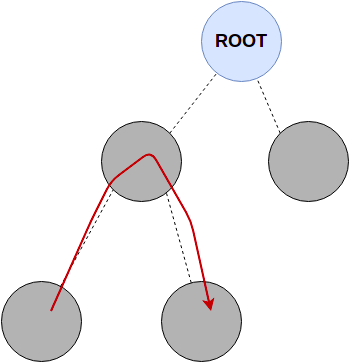
\includegraphics[scale=0.4]{res/pictures/rpl-storing.drawio.png}
            \caption{Storing.}
            \label{fig:state-path-storing}
        \end{subfigure}
        \caption{Chemin d'un paquet en fonction du MOP.}
        \label{fig:state-path-mop}
    \end{figure}

    Un noeud voulant rejoindre un DODAG doit être compatible avec le MOP du DODAG. Si ce n'est pas le cas, il doit rejoindre le DODAG comme feuille.



%\subsection*{Discussion}
%
%    D'après~\cite{paper:rpl-study}, après avoir été étudiés par le groupe de travail IETF roll %(Routing Over Low power and Lossy networks (roll), il s'est avéré que les protocoles tel que %OSPF, AODV ou OLSR ne satisfont pas toutes les exigences des LLNs. C'est pour cette raison que %ce groupe de travail a introduit RPL.
%
%    De plus, de part sa topologie et son fonctionnement, RPL est optimisé pour la collecte de %données ce qui est l'utilisation principale pour ce mémoire.

    %todo article qui regroupe plusieurs etudes: implémentation pas idéale dans COntiki mais article de 2017 -> corrigé depuis ??


%p9: peut bind un subnet
%p17: DODAG repair